\newpage
\section{The Road to Reality}

\subsection{Hyperbolic Geometry}
\bigskip

The ratio between the area \( A \) and \( A' \) of two similar shapes is given by
\[
	A' = k^2A
\]
\bigskip

\begin{theorem}[Pythagoras]\label{thm:thm_pythagoras}
	\[
		a^2 + b^2 = c^2
	\]
\end{theorem}


\begin{proof}
	Let \( A, B \) and \( C \) be the areas of the three triangles respectively. All triangles are similar, hence
	\[
		B = \frac{b^2}{a^2} A \text{ and }  C =  \frac{c^2}{b^2} B
	\]
	Since \( A + B = C \) it follows that
	\[
		a^2 + b^2 = \frac{b^2A}{B} + b^2 = \frac{b^2(A + B)}{B} = \frac{b^2 C}{B} = c^2
	\]
\end{proof}
\bigskip

% \begin{figure}[H]
% \centering
% \begin{tikzpicture}
% \plotrectriangle[black]{(0,0)}{(3,3)}{6cm}
% \end{tikzpicture}
% \caption{Pythagoras}\label{fig:pythagoras}
% \end{figure}
% \bigskip

\begin{lemma}[Conformal and Projective Representation]
	The mapping from conformal and projective representation of any point is given by the radial expansion of the following factor
	\[
		\frac{2R}{R^2 + r^2}
	\]
\end{lemma}

\begin{proof}
	For any point the distance from the origin with regard to the two representations is given by
	\[
		\log \frac{R + r}{R - r} = \frac{1}{2} \log \frac{R + r'}{R - r'} = \log \frac{{(R + r')}^2}{{(R - r')}^2}
	\]
	This gives
	\[
		{(R - r)}^2 (R + r') = {(R + r)}^2 (R - r') \text{ and } -4R^2r + 2R^2r' + 2r^2r' = 0
	\]
	Hence
	\[
		r' = \frac{2R^2}{R^2 + r^2} r
	\]
\end{proof}


\subsection{Complex Numbers}
\bigskip

\begin{lemma}[Basic Formulas]\hfill
	\begin{enumerate}
		\item It is
		      \[
			      (a + \iu b) (c + \iu d) = (ac - bd) + \iu (ad + bc)
		      \]
		\item Thus
		      \[
			      {(a + \iu b)}^2 = (a^2 - b^2) + \iu 2ab
		      \]
		      and
		      \[
			      (a + \iu b) (a - \iu b) =  a^2 + \iu ab - \iu ab - \iu^2b^2 = a^2 + b^2
		      \]
		\item Hence
		      \[
			      \frac{a + \iu b}{c + \iu d} = \frac{(a + \iu b)(c - \iu d)}{c^2 + d^2} =
			      \frac{ac + bd}{c^2 + d^2} + \iu \frac{bc - ad}{c^2 + d^2}
		      \]
		\item For
		      \[
			      z = \sqrt{\frac{1}{2}(a + \sqrt{a^2 + b^2})} + \iu \sqrt{\frac{1}{2}(-a + \sqrt{a^2 + b^2})}
		      \]
		      it follows
		      \[
			      z^2 = \frac{1}{2}(a + \sqrt{a^2 + b^2}) - \frac{1}{2}(-a + \sqrt{a^2 + b^2}) +
			      \iu 2\sqrt{\frac{1}{4} (\sqrt{a^2 + b^2}^2) - a^2} = a + \iu b
		      \]
		\item The complex conjugation \( \bar{z} = a - \iu b \) gives
		      \[
			      \Re z = \frac{z + \bar{z}}{2} \fspace \Im z = \frac{z - \bar{z}}{2\iu}
		      \]
	\end{enumerate}
\end{lemma}
\bigskip


\begin{lemma}[Binomial Theorem]\hfill
	\begin{enumerate}
		\item For the binomial coefficient Pascal's identity holds
		      \[
			      \binom{n}{k - 1} + \binom{n}{k} = \binom{n + 1 }{k }
		      \]
		\item The following equation states the binomial identity
		      \[
			      {(a + b)}^n = \sum_{k=0}^{n} \binom{n}{k} a^{k} b^{n - k} = \sum_{k=0}^{n} \binom{n}{k} a^{n -k} b^{k}
		      \]
		\item For \( a = 1 \) follows
		      \[
			      {(1 + x)}^n = \sum_{k=0}^{n} \binom{n}{k} x^{k}
		      \]
	\end{enumerate}
\end{lemma}

\begin{proof}
	It is
	\[
		\binom{n}{k} + \binom{n}{k - 1} = \frac{n!}{k!(n - k)!} + \frac{n!}{(k - 1)!(n - k + 1)!}
		= \frac{n!(n + 1 - k) + n!k!}{k!(n + 1- k)!} = \binom{n + 1}{k}
	\]
	Furthermore by using induction
	\[
		\begin{split}
			{(a + b)}^{n + 1}	& = \sum_{k=0}^{n} \binom{n}{k} a^{k + 1} b^{n - k} +
			\sum_{k=0}^{n} \binom{n}{k} a^{k} b^{n + 1 - k} \\
			& = \sum_{k=1}^{n + 1} \binom{n}{k - 1} a^{k} b^{n + 1 - k} +
			\sum_{k=0}^{n} \binom{n}{k} a^{k} b^{n + 1 - k} \\
			& = \sum_{k=0}^{n + 1} \binom{n + 1}{k} a^{k} b^{n + 1 - k}
		\end{split}
	\]
\end{proof}
\bigskip


\subsection{Exponential Function and Logarithms}
\bigskip

\begin{exercise}[Exponential Function]
	The Cauchy product yields
	\[
		\sum_{n=0}^\infty a_n \sum_{n=0}^\infty b_n = \sum_{n=0}^\infty \sum_{k=0}^n a_k b_{n-k}
	\]
	if at least one of the series is absolutely convergent. Hence
	\[
		\begin{split}
			\sum_{n=0}^\infty \frac{1}{n!} z^n \sum_{n=0}^\infty \frac{1}{n!} w^n
			& = \sum_{n=0}^{\infty} \sum_{k=0}^{n} \frac{1}{k!} z^{k} \frac{1}{(n - k)!} w^{n - k} \\
			& = \sum_{n=0}^{\infty} \frac{1}{n!} \sum_{k=0}^{n} \binom{n}{k} z^{k}w^{n - k} \\
			& = \sum_{n=0}^\infty \frac{1}{n!} {(z + w)}^n
		\end{split}
	\]
\end{exercise}
\bigskip


Let \( t \in \R \). Then
\[
	\begin{split}
		\eu^{\iu t}
		& = \sum_{k=0}^\infty \frac{1}{k!} {(\iu t)}^k \\
		& = \sum_{k=0}^\infty \frac{1}{2k!} {(\iu t)}^{2k} +
		\sum_{k=0}^\infty \frac{1}{(2k + 1)!} {(\iu t)}^{2k + 1} \\
		& = \sum_{k=0}^\infty \frac{{(-1)}^k}{2k!} t^{2k} +
		\iu\sum_{k=0}^\infty \frac{{(-1)}^k}{(2k + 1)!} t^{2k + 1} \\
		& = \cos{t} + \iu\sin{t}
	\end{split}
\]

More generally for \( z = \log r + \iu t\)
\[
	\eu^z = \eu^{\log r + \iu t} = r\eu^{\iu t} = r(\cos{t} + \iu\sin{t})
\]

For \( r = 1 \) and \( t = 2\pi \) this yields
\[
	\eu^{2\pi\iu} = \cos{2\pi} + \iu \sin{2\pi} = 1
\]
and for \( t = 2\pi \) it follows
\bigskip

\begin{lemma}[Euler Equation]\label{lemma:lemma_euler_equation}
	\[
		\eu^{\pi\iu} + 1 = 0
	\]
\end{lemma}
\bigskip


\begin{exercise}\hfill
	\begin{enumerate}
		\item If \( \eu^z = w \) then \( z + \pi\iu \) is a logarithm to \( -w \):
		      \( \eu^{z + \pi\iu} = \eu^{z}\eu^{\pi\iu} = - \eu^{z} = -w \).
		\item Since \( \eu^{i(s + t)} = \eu^{is} \eu^{it} \) it follows
		      \[
			      \begin{split}
				      \cos{(s + t)} + \iu \sin{(s + t)}
				      & = (\cos{s} + \iu\sin{s})(\cos{t} + \iu\sin{t}) \\
				      & = \cos{s}\cos{t} - \sin{s}\sin{t} + \iu(\cos{s}\sin{t} + \sin{s}\cos{t})
			      \end{split}
		      \]
		      Hence
		      \[
			      \begin{split}
				      \cos{(s + t)} & = \cos{s}\cos{t} - \sin{s}\sin{t} \\
				      \sin{(s + t)} & = \cos{s}\sin{t} + \sin{s}\cos{t}
			      \end{split}
		      \]
		\item It is \( \eu^{3it} = {(\eu^{it})}^3 \) and thus
		      \[
			      \cos{3t} + \iu \sin{3t}
			      = {(\cos{t} + \iu\sin{t})}^3
			      = \cos^3{t} - 3\cos{t}\sin^2(t) + \iu(\cos^2{t}\sin{t} -\sin^3{t})
		      \]
		\item Fun facts
		      \[
			      \eu^{1 - 4\pi^2} = \eu^{1 + {(2\iu\pi)}^2} = \eu \eu^{2\pi\iu}\eu^{2\pi\iu} = \eu
		      \]
		      and \( \iu = \eu^{\iu\pi/2} \) gives
		      \[
			      \iu^\iu = \eu^{\iu\log\iu} = \eu^{\iu\iu\pi/2} = \eu^{-\pi/2} \in \R
		      \]
	\end{enumerate}
\end{exercise}
\bigskip


\subsection{Complex Analysis}
\bigskip

\begin{definition}[holomorphic Function]\label{def:holomorphic_fnc}
	Let \( \Omega \subseteq \C \) be open. A function \( f : \Omega \to \C \) is called \emph{differentiable} at
	\( z \in \Omega \) if the limit
	\[
		f'(z) = \lim_{h \to 0} \frac{f(z + h) - f(z)}{h}
	\]
	exists. \( f \) is called \emph{holomorphic} on \( \Omega \) if \( f \) is complex differentiable
	at all points of \( \Omega \) and \( f': \Omega \to \C \) is called the \emph{derivative} of \( f \).
\end{definition}
\bigskip

\begin{remarks}\hfill
	\begin{enumerate}
		\item \( f \) is differentiable at \( z_0 \in \Omega \) iff the limit
		      \[
			      f'(z_0) = \lim_{z \to z_0}  \frac{f(z) - f(z_0)}{z - z_0}
		      \]
		      exists
		\item
		      If \( f \) is differentiable at \( z_0 \in \Omega \) and \( \eps > 0 \) then there exists a small
		      enough environment of \( z_0 \) so that
		      \[
			      | f(z) - f(z_0) - f'(z_0)(z - z_0)| < \eps |z - z_0|
		      \]
	\end{enumerate}
\end{remarks}
\bigskip


\begin{theorem}[Cauchy Riemann Equations]\label{thm:thm_cauchy_riemann_eqations}
	Let \( f = u + \iu v \) be holomorphic. Then \( f \) satisfies the Cauchy Riemann equations
	\[
		\frac{\partial u}{\partial x} = \frac{\partial v}{\partial y}
	\]
	\[
		\frac{\partial u}{\partial y} = - \frac{\partial v}{\partial x}
	\]
\end{theorem}

\begin{proof}
	For \( h \in \R \) follows
	\[
		\lim_{h \to 0}\frac{f(z + h) - f(z)}{h} = \frac{\partial u}{\partial x}(z) + \iu \frac{\partial v}{\partial x}(z)
	\]
	and
	\[
		\lim_{h \to 0}\frac{f(z + \iu h) - f(z)}{\iu h}
		= \frac{\partial u}{\iu\partial y}(z) + \frac{\partial v}{\partial y}(z)
		= \frac{\partial v}{\partial y}(z) - \iu\frac{\partial u}{\partial y}(z)
	\]

\end{proof}
\bigskip


\begin{examples}\hfill
	\begin{enumerate}
		\item Let \( f(z) = z^3 \). Then \( u(x,y) + \iu v(x,y) = x^3 - 3xy^2 + \iu (3x^2y -y^3) \) and as expected
		      \[
			      \begin{split}
				      \frac{\partial u}{\partial x}(x,y) = x^3 - 3y^2 & \quad\text{ and }\quad
				      \frac{\partial u}{\partial y}(x,y) = -6xy \\
				      \frac{\partial v}{\partial x}(x,y) = 6xy & \quad\text{ and }\quad
				      \frac{\partial v}{\partial y}(x,y) = x^3 - 3y^2
			      \end{split}
		      \]
	\end{enumerate}
\end{examples}
\bigskip


\begin{lemma}
	Let \( D \subseteq \C \) be connected. For arbitrary \( z, w \in D \) there exists a polygonal path from
	\( z \) to \( w \).
\end{lemma}
\begin{proof}
	For any path from \( z \) to \( w \) the image is compact, which can be used to define a finite subcover of disks.
	Use the center points to define the polygonal path.
\end{proof}
\bigskip


\begin{lemma}
	Let \( \gamma: [a,b] \to \C \) a smooth path, \( \psi: [c,d] \to [a,b] \) a smooth and increasing bijection
	and \( f \) continous.
	\[
		\int_{\gamma} f(z)\,dz = \int_{\gamma\circ\psi} f(z)\,dz
	\]
\end{lemma}

\begin{proof} It is
	\[
		\begin{split}
			\int_{\gamma\circ\psi} f(z)\,dz
			& = \int_c^d f(\gamma\circ\psi(t))(\gamma\circ\psi)'(t)) \,dt \\
			& = \int_{\psi(a)}^{\psi(b)} f(\gamma(\psi(t))\gamma'(\psi(t))\psi'(t) \,dt \\
			& = \int_a^b f(\gamma(s))\gamma'(s) \,ds = \int_{\gamma} f(z)\,dz
		\end{split}
	\]
\end{proof}
\bigskip


\begin{lemma}
	For a smooth path \( \gamma: [a,b] \to \C \) define \(-\gamma(t) = \gamma(a + b - t) \).
	Then
	\[
		\int_{-\gamma} f(z)\,dz = -\int_{\gamma} f(z)\,dz
	\]
\end{lemma}

\begin{proof} Using integration by substitution
	\[
		\int_{-\gamma} f(z)\,dz
		= - \int_a^b f(\gamma(a + b - t))\gamma'(a + b - t)) \,dt
		= \int_b^a f(\gamma(s))\gamma'(s) \,ds
		= - \int_{\gamma} f(z)\,dz
	\]
\end{proof}
\bigskip


In order to use the results from real calculus recall the fact, that for every \( z \in \C \)
there exists a \( t \in [0,2\pi] \) so that \( z = |z|e^{\iu t} \) and hence \( |z| = ze^{-\iu t} \).
\bigskip


\begin{lemma}
	Let \( f \in C[a,b] \). Then
	\[
		\left|\int_a^b f(x)\,dx \right| \le \int_a^b |f(x)|\,dx
	\]
\end{lemma}

\begin{proof} Using the estimation for integrals from real calculus
	\[
		\left|\int_a^b f(x)\,dx \right|  = e^{-\iu t}\int_a^b f(x)\,dx \le \int_a^b |e^{-\iu t}f(x)|\,dx
		= \int_a^b |f(x)|\,dx
	\]
\end{proof}
\bigskip


Let \( \gamma: [a,b] \to \C \) be a smooth path and \( a = t_0 < t_1 < \cdots < t_n = b \)
a partioning of \( [a,b] \). Then
\[
	\sum_{k = 1}^n |\gamma(t_k) - \gamma(t_{k - 1})|
	= \sum_{k = 1}^n \left| \frac{\gamma(t_k) - \gamma(t_{k - 1})}{t_k - t_{k - 1}} \right| (t_k - t_{k - 1})
	= \sum_{k = 1}^n | \gamma'(\xi_k)| (t_k - t_{k - 1})
\]
yields a reasonable approximation of the length of the path. Hence
\bigskip


\begin{definition}
	For a smooth path \( \gamma: [a,b] \to \C \)
	\[
		L(\gamma) = \int_a^b |\gamma'(t)|\,dt
	\]
	is called the length of \( \gamma \).
\end{definition}
\bigskip


\begin{lemma}[Estimation Lemma]
	Let \( \gamma: [a,b] \to \C \) be a smooth path. Then
	\[
		\left| \int_{\gamma} f(z)\,dz \right| \le L(\gamma) \max_{\gamma[a.b]} f
	\]
\end{lemma}

\begin{proof} Using the definition above
	\[
		\left| \int_{\gamma} f(z)\,dz \right|
		= \left| \int_a^b f(\gamma(t))\gamma'(t)\,dt \right|
		\le \int_a^b |f(\gamma(t))\gamma'(t)|\,dt
		\le  \max_{\gamma[a.b]}f \int_a^b |\gamma'(t)|\,dt
	\]
\end{proof}
\bigskip


\begin{examples}\hfill
	\begin{enumerate}
		\item Let \( \gamma(t) = t + \iu t \). Then
		      \[
			      \int_{\gamma} z^2\,dz
			      = \int_0^1 {(t + \iu t)}^2(1 + \iu)\,dt
			      = (1 + \iu)\int_0^1 2\iu t^2\,dt
				      = {\left[ (-2 + 2\iu) t^2 \right]}_0^1
			      = -\frac{2}{3} + \iu \frac{2}{3}
		      \]
		\item For \( \gamma(t) = t^2 + \iu t \)
		      \[
			      \begin{split}
				      \int_\gamma z^2\,dz
				      & = \int_0^1 {(t^2 + \iu t)}^2(2 + \iu t)\,dt = \int_0^1 (2t^5 - 4t^3) + \iu(5t^4 - t^2t)\,dt \\
				      & = {\left[ \frac{1}{3} t^6 - t^4 \right]}_0^1 + \iu {\left[ t^5 - \frac{1}{3}t^3 \right]}_0^1
				      = -\frac{2}{3} + \iu \frac{2}{3}
			      \end{split}
		      \]
		\item And \( \gamma(t) = \iu + \eu^{\iu t} \)
		      \[
			      \begin{split}
				      \int_\gamma z^2\,dz
				      & = \int_{3/2\pi}^{2\pi} {(\iu + \eu^{\iu t})}^2\iu\eu^{\iu t}\,dt
				      = \int_{3/2\pi}^{2\pi} (-1 + 2\iu\eu^{\iu t} + \eu^{2\iu t})\iu\eu^{\iu t}\,dt \\
				      & = \int_{3/2\pi}^{2\pi} -\iu\eu^{\iu t} - 2\eu^{2\iu t} + \iu\eu^{3\iu t}\,dt
					      = {\left[ -\eu^{\iu t} + \iu\eu^{2\iu t} + \frac{1}{3}\eu^{3\iu t}\right]}_{3/2\pi}^{2\pi} \\
				      & = \left( -1 + \iu + \frac{1}{3} \right) - \left( \iu - \iu + \frac{1}{3}\iu \right)
				      = -\frac{2}{3} + \iu \frac{2}{3}
			      \end{split}
		      \]
		\item Let \( \gamma(t) = \eu^{\iu t} \) and \( k \ne -1 \). Then
		      \[
			      \int_\gamma z^k\,dz =
			      \int_0^{2\pi} \eu^{\iu kt}\iu\eu^{\iu t}\,dt =
			      \int_0^{2\pi} \iu\eu^{\iu (k + 1) t}\,dt = 0
		      \]
	\end{enumerate}
\end{examples}
\bigskip


\begin{theorem}\label{thm:thm_antiderivative}
	Let \( D \subseteq \C \) be a connected domain and \( f \in C(D)\). Then the following assertions are equivalent
	\begin{enumerate}
		\item \( f \) has an antiderivative
		\item For every closd path \( \gamma \)
		      \[
			      \int_{\gamma} f(z)\,dz = 0
		      \]
	\end{enumerate}
\end{theorem}

\begin{proof} Let \( F' = f \). Since \( \gamma \) is closed
	\[
		\int_\gamma f(z)\,dz
		= \int_a^b f(\gamma(t))\gamma'(t)\,dt
		= \int_a^b (F\circ\gamma)'(t)\,dt
		= F(\gamma(b)) - F(\gamma(a)) = 0
	\]
	Now fix some arbitrary \( a \in D \). For \( z \in D \) let \( \gamma_z \) be a path from \( a \) to \( z \)
	and define
	\[
		F(z) = \int_{\gamma_z} f(\zeta)\,d\zeta
	\]
	This is well defined since the integral of \( f \) vanishes over each closed path. Moreover, since
	\( \gamma_{z + h} + [z + h,z] - \gamma_z \) defines a closed path
	\[
		F(z + h) - F(z)
		= \int_{\gamma_{z + h}} f(z)\,dz - \int_{\gamma_z} f(z)\,dz
		= \int_{[z,z + h]} f(z)\,dz
		= h\int_0^1 f(z + th)\,dt
	\]
	Here the latter integral is continous at \( 0 \) with respect to \( h \)
	\[
		\left|\int_0^1 f(z + th) - f(z)\,dt\right|
		\le \int_0^1 |f(z + th) - f(z)|\,dt
		\le \max_{t \in [0,1]}|f(z + th) - f(z)|
	\]
\end{proof}
\bigskip


\begin{corollary}The second assertion can be weakend to
	\[
		\int_{\boundary\Delta} f(z)\,dz = 0
	\]
	for every triangle \( \Delta \subset D\), where e.g. \( D \) is convex or star shaped. Here the antiderivative
	can directly be defined as
	\[
		F(z) = \int_{[a,z]} f(\zeta)\,d\zeta
	\]
	similar to the real calculus approach. Note, that under this conditions \( f \) always has a local antiderivative.
\end{corollary}
\bigskip


\begin{examples}\hfill
	\begin{enumerate}
		\item Let \( z_0 \in \C \) and \( \gamma(t) = z_0 + \eu^{\iu t} \) for \( t \in [0, 2\pi] \). Then
		      \[
			      \int_\gamma \frac{1}{z - z_0}\,dz
			      = \int_0^{2\pi} \frac{\iu \eu^{\iu t}}{z_0 + \eu^{\iu t} - z_0}\,dt
			      = \int_0^{2\pi} \iu \, dt
			      = 2\pi\iu
		      \]
		      and thus \( 1/ (z - z_0 ) \) has no antiderivative on \( \C \setminus \{z_0\} \)
		\item Let \( z_0 \in \C \) and \( z \in D = D_r(z_0) \). Applying
		      \hyperref[thm:thm_antiderivative]{Theorem~\ref*{thm:thm_antiderivative}}.
		      to \( \boundary D \) and a small enough circle around \( z \) gives
		      \[
			      \int_{\boundary D} \frac{1}{\zeta - z}\,d\zeta
			      = \int_{\boundary D} \frac{1}{\zeta - z_0}\,d\zeta
			      = 2\pi\iu
		      \]
	\end{enumerate}
\end{examples}
\bigskip


\begin{theorem}[Goursat]\label{thm:thm_goursat}
	Let \( \Omega \subseteq \C \) be open and \( f \) holomorphic on \( \Omega \).
	Then
	\[
		\int_{\boundary\triangle} f(z)\,dz = 0
	\]
	for every triangle \( \triangle \subset \Omega \).
\end{theorem}

\begin{proof}
	Choose a sequence of triangles \( \triangle \supset \triangle_0 \supset \triangle_1 \dots \supset \triangle_k \)
	as depicted. Since all the triangles are compact with a vainishing diameter there exists a unique \( z_0 \in \Omega \) with \( \bigcap \triangle_k = \{ z_0 \}  \). Thus
	\[
		\left| \int_{\boundary\triangle} f(z)\,dz \right|
		\le 4^k \left| \int_{\boundary\triangle_k} f(z)\,dz \right| \\
		= 4^k \left| \int_{\boundary\triangle_k} f(z) - f(z_0) - f'(z_0)(z - z_0)\,dz \right| \\
	\]
	Furthermore \( L(\boundary\triangle) = 2^{-k} L(\boundary\triangle_k) \) and
	\[
		|z - z_0| < L(\boundary\triangle_k) = 2^{-k} L(\boundary\triangle)
	\]
	for any \( z \in \triangle_k \). Since \( f \) is holomorphic at \( z_0 \) for any given \( \eps > 0 \)
	there exists a sufficiently large enough \( k \) so that
	\[
		\begin{split}
			\left| \int_{\boundary\triangle} f(z)\,dz \right|
			& \le 4^k L(\boundary\triangle_k) \max_{z \in \triangle_k} |f(z) - f(z_0) - f'(z_0)(z - z_0)| \\
			& \le 4^k L(\boundary\triangle_k) \,\eps \max_{z \in \triangle_k} |z - z_0| \\
			& \le {L(\boundary\triangle)}^2 \,\eps
		\end{split}
	\]
\end{proof}
\bigskip


\begin{corollary}\hfill
	\begin{enumerate}
		\item A holomorphic function always has a local antiderivative
		\item A holomorphic function on a star shaped domain has a global antiderivative and
		      \[
			      \int_{\gamma} f(z)\,dz = 0
		      \]
		      for any closed path
		\item The prerequites of Goursat theorem can be weakened to continous and holomorphic with
		      the exception of a finite number of points: adequate partioning of the original triangle
	\end{enumerate}
\end{corollary}
\bigskip


\begin{theorem}[Cauchy's Intergral Formula]
	Let \( \Omega \subseteq \C \) be open and \( f \) holomorphic on \( \Omega \). Further let \( D \subset \Omega \)
	be a disc. Then
	\[
		f(z) = \frac{1}{2\pi\iu} \int_{\boundary D} \frac{f(\zeta)}{\zeta - z}\,dz% \text{ for } z \in D
	\]
	for \( z \in D \).
\end{theorem}

\begin{proof}
	For \( z \in D \) define
	\[
		h(\zeta) = \frac{f(\zeta)- f(z)}{\zeta - z} % \text{ for } \zeta \ne z \text{ and } f'(z) \text{ for } \zeta = z
	\]
	for \( \zeta \ne z \) and \( f'(z)  \) for \( \zeta = z \). Then \( h \) is holomorphic on \( D \setminus \{ z \} \) and
	continous at \( z \)
	\[
		0 = \int_{\boundary D} h(\zeta) \,d\zeta
		= \int_{\boundary D} \frac{f(\zeta)}{\zeta - z}\,d\zeta - f(z)\int_{\boundary D} \frac{1}{\zeta - z}\,d\zeta
		= \int_{\boundary D} \frac{f(\zeta)}{\zeta - z}\,d\zeta - 2\pi\iu f(z)
	\]
\end{proof}
\bigskip


\subsection{Fourier Analysis}
\bigskip

\begin{lemma}
	Let \( u(x, t) = \sin(nx) \cos(nt) \) for some \( n \in \Z \). Then the \emph{wave equation} as well as
	the \emph{initial condition} and the \emph{boundary conditions} hold.
	\[
		\frac{\partial^2 u}{\partial x^2} = \frac{\partial^2 u}{\partial t^2} \fspace
		\frac{\partial u}{\partial t}(x, 0) = 0 \fspace
		u(0, t) = u(\pi, t) = 0
	\]
\end{lemma}

\begin{proof}
	It is \( \partial_x u(x, t) = n \cos(nx) \cos(nt) \) and \( \partial_t u(x, t) = -n \sin(nx) \sin(nt) \).
\end{proof}
\bigskip


\begin{lemma}
	For \( m, n \in \Z \)
	\begin{enumerate}
		\item
		      \[
			      \int_{-\pi}^\pi \cos(mx)\,dx = \int_{-\pi}^\pi \sin(nx)\,dx =  0
		      \]
		\item Here \( m \ne 0 \)
		      \[
			      \int_{-\pi}^\pi \cos^2(mx)\,dx = \int_{-\pi}^\pi \sin^2(nx)\,dx = \pi
		      \]
		\item
		      \[
			      \int_{-\pi}^\pi \cos(mx)\sin(nx)\,dx = \int_{-\pi}^\pi \sin(mx) \sin(nx)\,dx
			      = \int_{-\pi}^\pi \cos(mx) \cos(nx)\,dx = 0
		      \]
	\end{enumerate}
\end{lemma}

\begin{proof}
	For example
	\[
		\int_{-\pi}^\pi \sin^2(nx)\dx = {\left[\frac{1}{2}(x - \frac{1}{n}\cos(nx)\sin(nx))\right]}_{-\pi}^\pi = \pi
	\]
	The trigonometric identity \( 2\sin(x)\cos(y) = \sin(x - y) + \sin(x + y) \) gives
	\[
		\int_{-\pi}^\pi \cos(mx)\sin(nx)\,dx = \frac{1}{2} \int_{-\pi}^\pi \sin(nx - mx) + \sin(nx + mx)\dx = 0
	\]
\end{proof}
\bigskip


\begin{lemma}
	Let \( f \) be of the form
	\[
		f(x) = a_0 + \sum_{k = 1}^n a_k \cos(kx) + b_k \sin(kx)
	\]
	Then
	\[
		a_0 = \frac{1}{2\pi} \int_{-\pi}^\pi f(x)\,dx \fspace
		a_k = \frac{1}{\pi} \int_{-\pi}^\pi f(x)\cos(kx)\,dx \fspace
		b_k = \frac{1}{\pi} \int_{-\pi}^\pi f(x)\sin(kx)\,dx
	\]
\end{lemma}

\begin{proof}
	This follows from the previous lemma.
\end{proof}
\bigskip


\begin{example}
	Consider the absolute value function \( f(x) = |x| \). Then
	\[
		a_0 = \frac{1}{2\pi} \int_{-\pi}^\pi |x|\dx = \frac{1}{\pi} \int_0^\pi x\dx
		= \frac{1}{\pi} {\left[ \frac{x^2}{2} \right]}_{0}^\pi = \frac{\pi}{2}
	\]
	and
	\[
		a_k = \frac{1}{\pi} \int_{-\pi}^\pi |x|\cos(kx)\dx = \frac{2}{\pi} \int_0^\pi x\cos(kx)\dx
		= \frac{2}{\pi} {\left[ \frac{x}{n} \sin(nx) + \frac{1}{n^2} \cos(nx) \right]}_0^\pi
		% = \left\{
		% \begin{array}{ll}
		% 	-4/{\pi k^2} & k \text{ odd }  \\
		% 	0            & k \text{ even }
		% \end{array}
		% \right.
	\]
	Hence \( a_k = -4/{\pi k^2} \) for \( k \) odd and \( a_k = 0 \) otherwise. Furthermore
	\[
		b_k = \frac{1}{\pi} \int_{-\pi}^\pi |x|\sin(kx)\dx = 0
	\]
	since the integrand is odd. Now let
	\[
		S_n(x) = \frac{\pi}{2} - \frac{4}{\pi} \sum_{k=0}^n \frac{\cos((2k + 1)x)}{{(2k + 1)}^2}
	\]
	\begin{figure}[h!]
		\centering
		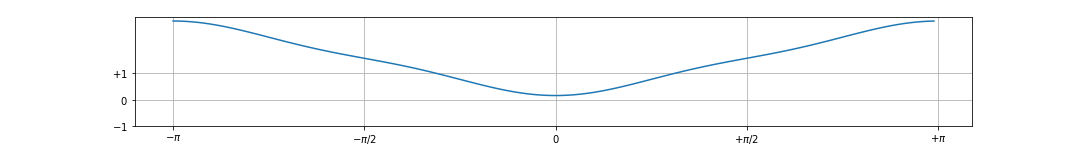
\includegraphics[width=\textwidth]{abs_value_n=2}
		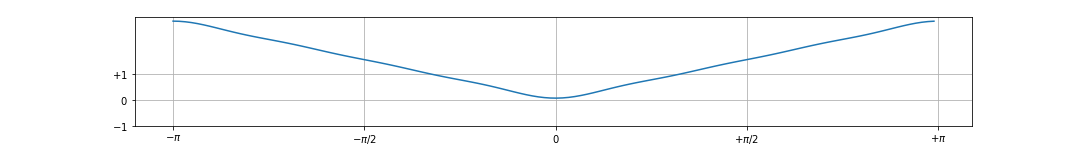
\includegraphics[width=\textwidth]{abs_value_n=4}
		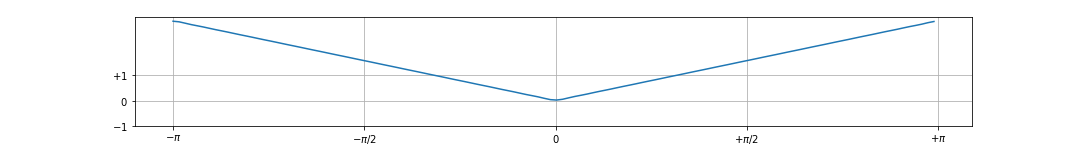
\includegraphics[width=\textwidth]{abs_value_n=16}
		\caption{Approximation absolute value function for \( n = 2, 4, 16 \)}
	\end{figure}
\end{example}
\bigskip


\begin{remarks}\hfill
	\begin{enumerate}
		\item
		      It is
		      \[
			      \cos x = \frac{1}{2} (\eu^{\iu x} + \eu^{-\iu x}) \fspace
			      \sin x = -\frac{\iu}{2} (\eu^{\iu x} - \eu^{-\iu x})
		      \]
		      Therefore
		      \[
			      \begin{split}
				      \frac{a_0}{2} + \sum_{k = 1}^n a_k \cos(kx) + b_k \sin(kx)
				      & = \frac{a_0}{2} + \sum_{k = 1}^n \frac{a_k}{2} (\eu^{\iu kx} + \eu^{-\iu kx}) -
				      \frac{\iu b_k}{2} (\eu^{\iu kx} - \eu^{-\iu kx}) \\
				      & = \frac{a_0}{2} + \sum_{k = 1}^n \frac{a_k - \iu b_k}{2} \eu^{\iu kx} +
				      \sum_{k=1}^n\frac{a_k + \iu b_k}{2} \eu^{-\iu kx} \\
				      & = \sum_{k=-n}^n c_k \eu^{\iu kx}
			      \end{split}
		      \]
		      where
		      \[
			      c_0 = \frac{a_0}{2} \fspace c_k = \frac{a_k - \iu b_k}{2} \fspace c_{-k} = \frac{a_k + \iu b_k}{2}
		      \]
		\item Thus for
		      \[
			      f(x) = \sum_{k=-n}^n c_k \eu^{\iu kx}
		      \]
		      it is
		      \[
			      c_k = \frac{1}{2\pi} \int_{-\pi}^\pi f(x) \eu^{-\iu kx}\dx
		      \]

	\end{enumerate}
\end{remarks}
\bigskip


\begin{definition}[Fourier Series]
	Let \( f \) be Riemann integrable over \( [-\pi,\pi] \). Then
	\[
		c_k = \frac{1}{2\pi} \int_{-\pi}^\pi f(x) \eu^{-\iu kx}\dx
	\]
	are called the \emph{Fourier coefficients} and
	\[
		F(x) = \sum_{k=-\infty}^\infty c_k \eu^{\iu kx}
	\]
	is called the \emph{Fourier series} of \( f\) wherever limit exists.
\end{definition}
\bigskip


